\documentclass{article} % For LaTeX2e
\usepackage{nips15submit_e,times}
\usepackage{hyperref}
\usepackage{url}
\usepackage{graphicx}
%\documentstyle[nips14submit_09,times,art10]{article} % For LaTeX 2.09


\title{Mid-Term Report - Prediction of Grant Applications}


\author{
Priyaranjan Behera\\
Department of Computer Science\\
North Carolina State University\\
\texttt{pbehera@ncsu.edu} \\
\And
Sai Sri Harsha Kunapareddy\\
Department of Computer Science\\
North Carolina State University\\
\texttt{skunapa@ncsu.edu} \\
}

% The \author macro works with any number of authors. There are two commands
% used to separate the names and addresses of multiple authors: \And and \AND.
%
% Using \And between authors leaves it to \LaTeX{} to determine where to break
% the lines. Using \AND forces a linebreak at that point. So, if \LaTeX{}
% puts 3 of 4 authors names on the first line, and the last on the second
% line, try using \AND instead of \And before the third author name.

\newcommand{\fix}{\marginpar{FIX}}
\newcommand{\new}{\marginpar{NEW}}

\nipsfinalcopy % Uncomment for camera-ready version

\begin{document}


\maketitle

\section{Background}

Around the world, the pool of funds available for research grants is steadily shrinking (in a relative sense). In Australia, success rates have fallen to 20-25 per cent, meaning that most academics are spending valuable time making applications that end up being rejected. This problem was hosted as a competition by University of Melbourne to address their inefficiencies with the grant applications. There is also a hope of discovering the most important criteria that are required to succeed in a grant application. 

\subsection{Problem}

The university has provided a dataset containing 249 features, including variables that represent the size of the grant, the general area of study and de-identified information on the investigators who are applying for the grant. The dataset contains multi-variate data with a few of them being continuous variable and a few categorical. There is a variable number of investigators in an application and thus, we need to aggregate the person data to create an efficient model. We are looking into implementing several of the classification techniques covered in the CSC522 course to arrive upon an efficient model.


\subsection{Literature Survey}

The dataset contains a variable number of person attributes for each of the investigators in an grant application. This would lead to multiple missing data fields in applications where the investigator count is less. According to Gerhard Svolba \cite{OneRow}, we need to create a one-row-per-subject data mart for most of the analytical methods that we need to proceed with. Accordingly, we need to aggregate the person data using mean, median, standard deviation, the quartiles, or special quantiles, etc to create the input rows.

We looked at approaches taken to solve similar problems which contains both continuous and categorical data \cite{Matlab} and found that decision trees and naive bayes are popular choices. On the contrary, methods like neural networks, SVM, etc. cannot work with categorical data. We will be looking to implement decision trees as well as bagged and boosted trees for more efficiency. 

Daniele et al. \cite{HighCard} focused on the transformation of categorical data to continuous/binary data so that we can use the analytical methods which cannot process categorical data. While traditionally 1-to-n encoding is used for conversion of categorical data to binary, for categories with high cardinality a probabilistic approach is suggested.

\section{Methods}

The analysis of the data required extensive preprocessing steps because of its multi-variate nature and variable number of attributes. We look to implement different type of classification techniques to compare the models and find the determining attributes for the classification.

\subsection{Preprocessing}

To handle the categorical values in the data, we indexed the attributes with numerical values after finding the unique values for each of the attributes. As per the approach suggested by Gerhard Svolba \cite{OneRow}, we aggregated the person data for each of the application which is not null and found the minimum, maximum for all the attributes. While for continuous attributes we also calculated mean, median, sum of the values to create new features. We then created plots of the attributes with respect to the output to visually inspect any correlation of the attributes with the results.

Since many of the classification techniques cannot handle categorical data, we look to implement 1-to-n encoding to convert the categorical data into binary attributes which can be used in the analytical techniques. Further, to handle high cardinality, we will implement a probabilistic feature creation as specified at \cite{HighCard}. 

\subsection{Classification}

We look to implement most of the classification techniques covered in CSC522 and compare their efficiencies.

\subsubsection{Decision Tree and Random Forest}
According to our survey of approaches employed for similar problems, decision tree turns out to be a popular choice. This attributes to the fact the it can handle categorical values without any further processing. We also implemented bagged trees using the dataset to get a more efficient classification. We also can use the decision tree to determine the most important factors which decide the success of a grant application.

\subsubsection{Neural Networks}
Since the neural networks can handle a high number of attributes, this will serve as an ideal classifier particularly when we use the 1-to-n encoding with a high cardinality of the categorical attributes. However, we cannot estimate the determining factors of an application though this method.

\subsubsection{Naive Bayes}
Since categorical variables can also be handled by the Naive Bayes approach, we will use this classification method. However, we will extract the determining features by the use of the decision tree and use only a fraction of the features which has high effectiveness. 


\section{Plan}
According to the problem statement of the competition, we will be aiming to find a model which has a greater accuracy while minimizing the false positives in the output.

\subsection{Hypothesis}
We will work on implementing models of the classifications techniques we have been familiarized with to find a model with lesser number of false positives and higher accuracy. Thus, we will focus on the values of True Positive Rate, False Positive Rate, Precision and Accuracy of the models. Most importantly, we will be using the ROC (Receiver Operating Curve) to determine the effectiveness of the model by comparing the area under the curve for the models. This will be more helpful compared to other criteria as:
\begin{itemize}
	\item It is insensitive to unbalanced dataset where there is a disparity in the number of test cases outputs.  
	\item We consider all the cut-offs in a model to find its effectiveness.
\end{itemize}

We will work on experiments to test the technique of conversion of categorical attributes to probabilistic values for high cardinality attributes\cite{HighCard}. We will consider the same criteria mentioned above to compare models which use 1-to-n encoding. 

We will also look into finding of the most determining factors which decides the fate of an application. For this, we will use the characteristic of the random forest libraries which find the effective factors in an input. These important factors will later be used to create a naive bayes classifier.

\subsection{Experimental Design}
\begin{enumerate}
	\item \emph{Data Indexing:} Since there are a large number of categorical attributes in the data, indexing was done to standardize them into integral values.
	\item \emph{Dimensionality Reduction and Data Creation:} Since the data has variable number of person data in each of the grant application, there was a need to aggregate the data to create similar rows for comparing applications. We used different aggregation functions within a data row\cite{OneRow} to achieve this.
	\item \emph{Data Visualization:} Effectiveness of the attributes to determine the result of an application was studied by creating scatter plots and histograms for each of the attributes in the input matrix. 
	\item \emph{Handling of Categorical Attributes:} While techniques involving decision trees and naive bayes work well with categorical values, other methods need binary or continuous inputs. Thus, we will be adopting two methods 
	\begin{itemize}
		\item 1-to-n encoding
		\item probability substitution \cite{HighCard}
	\end{itemize}  
	
	to use the data in other classifiers.

	
	\item \emph{Classifications:} We will be using the different inputs obtained in the above steps to train and test the classifiers.
	\begin{itemize}
		\item Decision Tree
		\item Random Forest
		\item Neural Networks
		\item SVM
		\item Naive Bayes
	\end{itemize}
	 Primarily, libraries in Matlab will be used for this purpose where tools like 'classificationLearner', 'nprtool' will be used in addition to other basic classifier classes.
	 
	 \item \emph{Factor Determination:} The random forest library explicitly determines the most important factor which decides the output. We will be using this to find out the factors which can improve the credentials of an application.
	 
	 \item \emph{Evaluation and Results:} Confusion matrices will be drawn for each of the classification done in the experiments to find the accuracy, recall, precision and false positive rate. Additionally, ROC will be generated from the GUI interfaces in 'classificationLearner' and 'nprtool'.
	
	\end{enumerate}
	
	
\section{Experiments}

After the pre-processing steps which included indexing and generation of new features, we resorted to visualization of the data to find any correlation of attributes with the results (As shown in Fig.\ref{fig:sponsor}).

\begin{figure}[h]
	\begin{center}
		%\framebox[4.0in]{$\;$}
		\fbox{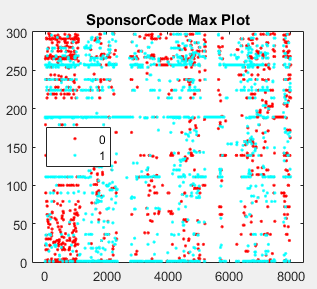
\includegraphics[scale=0.5]{SponsorPlot.png}}
		\fbox{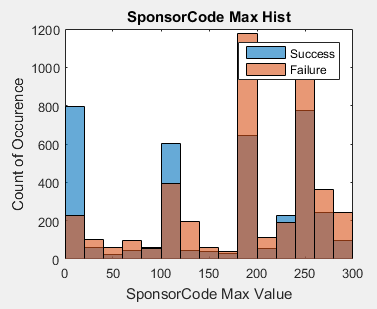
\includegraphics[scale=0.5]{SponsorHist.png}}
	\end{center}
	\caption{Scatter Plot and Histogram for Sponsor Codes.}
	\label{fig:sponsor}
\end{figure}

We take an example of Sponsor code here, for which we plot the data and see a discerning pattern. We can see that for specific sponsor codes, the chances of getting a grant is more.

But we could not find any conclusive pattern in any of the plots and thus, moved on with the classification. Since decision trees doesn't have much problem with the number of dimensions we moved ahead with building decision tree and random forest classifiers. For the decision tree classifier we opted for a 5-fold cross validation. The confusion matrix along with TPR/FPR rate for the random forest is listed at Fig.\ref{fig:RFCM}. The accuracy obtained for the decision tree is 82.6\% while for the random forest is 85.9\%.

\begin{figure}[h]
	\begin{center}
		%\framebox[4.0in]{$\;$}
		\fbox{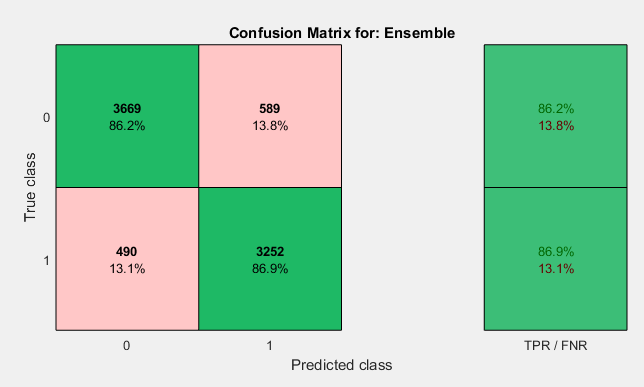
\includegraphics[scale=0.5]{RandomForestCM.png}}
	\end{center}
	\caption{Confusion Matrix and TPR/FPR of Random Forest.}
	\label{fig:RFCM}
\end{figure}

By comparing the models with respect to the ROC curve(Fig.\ref{fig:ROC}), we find that the area under the curve for random forest is a little high and thus, random forest is a better model in this scenario.

\begin{figure}[h]
	\begin{center}
		%\framebox[4.0in]{$\;$}
		\fbox{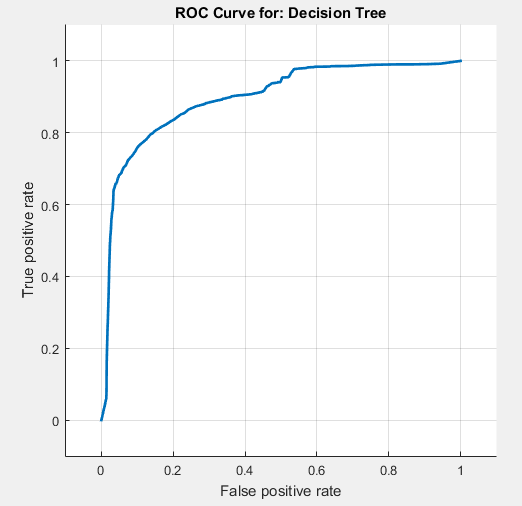
\includegraphics[scale=0.4]{ROC-DT.png}}
		\fbox{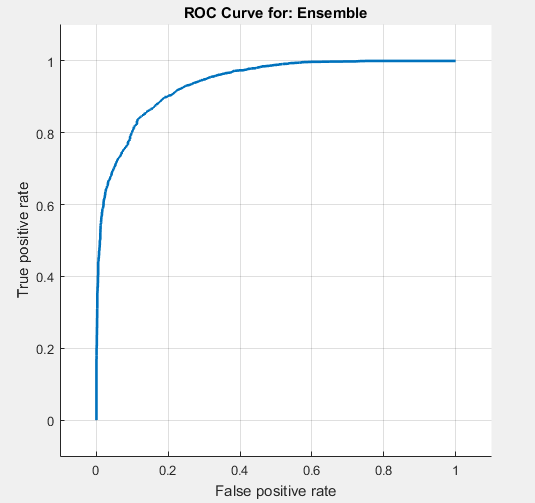
\includegraphics[scale=0.4]{ROC-RF.png}}
	\end{center}

	\caption{ROC Plot for Decision Tree and Random Forest.}
	\label{fig:ROC}
\end{figure}

In addition, we found the important features which determine the outcome of the application. The data is plotted in Fig.\ref{fig:FIM}. From the plot we can see that features Contract Value(3), Sponsor Code(1), Application Month(14), Grant Category(2) are the most important factors.

\begin{figure}[h]
	\begin{center}
		%\framebox[4.0in]{$\;$}
		\fbox{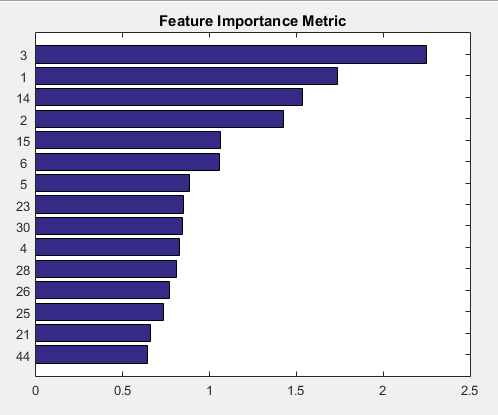
\includegraphics[scale=0.5]{FIM.png}}
	\end{center}
	\caption{Feature Importance Matrix Generated By Random Forest.}
	\label{fig:FIM}
\end{figure}


\section{Conclusion}
The experiments using the categorical values without encoding is done for decision tree and random forest, where we found random forest to be a little more accurate. Further, we will work on encoding the categorical attributes and create models based on neural networks, SVM and naive bayes classifiers.

\begin{thebibliography}{10} % 100 is a random guess of the total number of
	%references
	\bibitem{Top10} Top 10 algorithms in data mining. Knowl. Inf. Syst. 14, 1 (December 2007), 1-37. DOI=http://dx.doi.org/10.1007/s10115-007-0114-2
	\bibitem{OneRow} Efficient “One-Row-per-Subject” Data Mart Construction for Data Mining, Gerhard Svolba, PhD, SAS Austria
	\bibitem{Multi} Reliable Early Classification on Multivariate Time Series with Numerical and Categorical Attributes, Cao, Tru et al.
	\bibitem{HighCard}Daniele Micci-Barreca. 2001. A preprocessing scheme for high-cardinality categorical attributes in classification and prediction problems. SIGKDD Explor. Newsl. 3, 1 (July 2001), 27-32. DOI=http://dx.doi.org/10.1145/507533.
	\bibitem{Matlab} Getting Started with Kaggle Data Science Competitions. Loren Shure
	\bibitem{Matlab} Predict Grant Applications - Kaggle Competition, https://www.kaggle.com/c/unimelb 
\end{thebibliography}

\newpage
\appendix
\section{Appendix} \label{App:Appendix}
	\subsection{Deviation from Initial Proposal}
	In the proposal, we didn't focus more on the pre-processing steps, particularly encoding of the categorical attributes. After further work on the project, this became a necessity to implement the different kinds of classifiers. Thus, we are looking into implementing 1-to-n encoding and a probabilistic encoding after the mid-term report submission.
	
	We also found the way to extract the importance of features for the classification with the help of decision trees and random forest. Thus, our results will also include the features which will decide the classifications most. 
	
	\subsection{Division of Work}
	Priyaranjan and Harsha worked in the pre-processing steps and implementation of decision trees and random forest collaboratively. Going forward, Priyaranjan will work on the probabilistic encoding of categorical attributes and the classifications. While, Harsha will work on the 1-to-n encoding and the related classifications.

\end{document}
